\documentclass[a4paper,11pt]{article}
\usepackage{amsmath}
\usepackage{wrapfig}
\usepackage{fancyhdr}
\usepackage{graphicx}
\usepackage{url}
\usepackage{float}
\usepackage{amsmath}
\usepackage{amssymb}
\usepackage[margin=1in]{geometry}

%\setlength{\voffset}{-0.5in}
%\setlength{\headsep}{5pt}
\newcommand{\suchthat}{\;\ifnum\currentgrouptype=16 \middle\fi|\;}


%===========---------================
% Author John H Allard
% CMPE 12, Lab #2 Write-up
% October 9th, 2014
%===========---------================


\title{ CMPE 12 Homework \#1 \\[7 in]}
\author{John Allard \\ Lab Section \#2}
\date{October 20th, 2014}

\begin{document}
\maketitle
\newpage

%==========================================
%==========================================
%====== Begin Problems, 15 Total ==========
%==========================================
%==========================================

\begin{enumerate}
%==========================================
%========= Ch 1, #5 (1 pt) =============
%==========================================
\item If you had a black box that takes two inputs and adds them, and another black box that takes two numbers and multiplies them, can you combine these boxes in a certain way to create the functions given below?

  \begin{enumerate}

  % === Part A ===
  \item $ax+b$ \\
  \textbf{Answer :} $M(n_1, n_2) = n_1*n_2$, $A(n_1, n_2) = n_1+n_2$. Then $ax+b = A(M(a, x), b)$ 

   % === Part B ===
  \item The average of four input numbers, $w, x, y, z$ \\
  \textbf{Answer :} $\text{Average}(w, x, y, z) = M(\frac{1}{4}, A(w, A(x, A(y, z))))$

  % === Part C ===
  \item $a^2 + 2ab + b^2$ \\
  \textbf{Answer :} $a^2 + 2ab + b^2 = M(A(a,b), A(a,b)) $ 


  \end{enumerate}

%==========================================
%========= Ch 1, #13 (1 pt) =============
%==========================================
\item Two computers are identical except that the first one has no subtraction command, and the second one does. They both can add and take the negative of a given number, which is able to solve more problems? \\
\textbf{Answer :} The two machines can do exactly the same functions and can solve the exact same problems. There are two explanations for this, first, the Turing thesis which states that any two computers can perform the exact same calculations. This means that it might take one of the computers longer to perform a computation, but it can still perform everything that any other computer can. A more intuitive reason for this being true is that subtraction is equivelant to addition of a negative number. So the computer without the subtraction command can simply add the negative of the number that it is trying to subscribe. 

%==========================================
%========= Ch 1, #18 (1.5 pts) =============
%==========================================
\item Normally one ISA is implemented per microarchitecture. It is possible for many different varieties of microarchitectures to implement the same ISA though.

%==========================================
%========= Ch 2, #2 (1.5 pts) =============
%==========================================
\item We would need $\text{int}(\text{log}_2(26)+1) = 5$ bits to represent all 26 characters. If we wanted to also include lower case, we would need $\text{int}(\text{log}_2(52)+1) = 6$ bits. 

%==========================================
%========= Ch 2, #11 (1 pt) =============
%==========================================
\item Convert the following numbers to 8-bit two's compliment binary numbers.
  \begin{enumerate}
  %== a.) ==
  \item 102  \textbf{Answer :} 001100110

  %== b.) ==
  \item 64  \textbf{Answer :} 001000000

  %== c.) ==
  \item 33  \textbf{Answer :} 000100001

  %== d.) ==
  \item -128  \textbf{Answer :} 101111111

  %== e.) ==
  \item 127 \textbf{Answer :} 001111111
  \end{enumerate}

%==========================================
%========= Ch 2, #30 (1.5 pts) =============
%==========================================
\item Compute the following, write you results in binary.

  \begin{enumerate}
  %=== a.) ===
  \item 01010111 AND 11010111 \textbf{Answer :} 01010111
  %=== b.) ===
  \item 101 AND 110 \textbf{Answer :} 100
  %=== c.) ===
  \item 11100000 AND 10110100 \textbf{Answer :} 10100000
  %=== d.) ===
  \item 00011111 AND 10110100 \textbf{Answer :} 00010100
  %=== e.) ===
  \item (0011 AND 0110) AND 1101 \textbf{Answer :} 0000 
  %=== f.) ===
  \item 0011 AND (0110 AND 1101) \textbf{Answer :} 0000
  \end{enumerate}

%==========================================
%========= Ch 2, #34 (1.5 pts) =============
%==========================================
\item Compute the following :

  \begin{enumerate}
  %=== a.) ===
  \item NOT(1011) OR NOT(1100)  \textbf{Answer :} 0111  
  %=== b.) ===
  \item NOT(1000 AND (1100 OR 0101))  \textbf{Answer :}   0111
  %=== c.) ===
  \item  NOT(NOT(1101)) \textbf{Answer :}   1101
  %=== d.) ===
  \item  (0100 OR 0000) AND 1111 \textbf{Answer :}  0100
  \end{enumerate}

%==========================================
%========= Ch 2, #43 (1.5 pts) =============
%==========================================
\item Translate the following ASCII codes into strings of characters by interpreting each group of 8 bits as an ASCII character.

  
  \begin{enumerate}
  %=== a.) ===
  \item x48656c6c6f21  \textbf{Answer :}    Hello!
  %=== b.) ===
  \item  x68454c4c4f21 \textbf{Answer :}    Hello!
  %=== c.) ===
  \end{enumerate}


%==========================================
%========= Ch 2, #47 (1 pt) =============
%==========================================
\item Convert the following hexidecimal representation of two's compliment numbers in their binary form.
  
  \begin{enumerate}
  %=== a.) ===
  \item xF0  \textbf{Answer :}    1111 0000 = -(00001111) = -15
  %=== b.) ===
  \item x7FF \textbf{Answer :}    0111 1111 1111 = 2047
  %=== c.) ===
  \item x16  \textbf{Answer :}    0001 0110 = 22
  %=== d.) ===
  \item x8000  \textbf{Answer :}    1000 0000 0000 0000 = -(0111 1111 1111 1111) = -32,768
  \end{enumerate}

%==========================================
%========= Ch 2, #55 (1.5 pts) =============
%==========================================
\item We will now be working in quad (base-4). 

  \begin{enumerate}
  \item Max unsigned decimal value that can represented with 3 quad digits? \textbf{Answer :} $4^3$ = $64$
  \item Max unsigned ..... with $n$ quad digits? \textbf{Answer :} $4^n$
  \item Add the two unsigned quad numbers 023 and 221 \textbf{Answer :} 023$_4$ = 11$_{10}$. 221$_4$ = 41$_{10}$. 41+11 = 52$_{10}$
  \item What is the quad representation of 42 in quad? \textbf{Answer :} 42$_{10}$ = 222$_4$
  \end{enumerate}

%==========================================
%========= Ch 3, #5 (1.5 pts) =============
%==========================================
\item Complete a truth table for the transistor-level circuit in Figure 3.34 (Page 83, Textbook).
\textbf{Answer :} 
\begin{tabular}{ l | c | c | r }
  A & B & C & Out \\
  \hline 
  0 & 0 & 0 & 1 \\
  \hline
  0 & 0 & 1 & 0 \\
  \hline 
  0 & 1 & 0 & 1 \\
  \hline
  0 & 1 & 1 & 0 \\
  \hline 
  1 & 0 & 0 & 1 \\
  \hline
  1 & 0 & 1 & 0 \\
  \hline 
  1 & 1 & 0 & 0 \\
  \hline 
  1 & 1 & 1 & 0 \\
\end{tabular}

%==========================================
%========= Ch 3, #8 (1.5 pts) =============
%==========================================
\item The circuit in Figure \ref{fig:prob8} is implementing equation \eqref{eq:prob8}. Label the circuit to fit the equation.
\begin{equation} \label{eq:prob8} Y = \text{NOT}(A \text{ AND } (B \text{OR} C))
\end{equation}
\begin{figure}[h!]
   \centering
     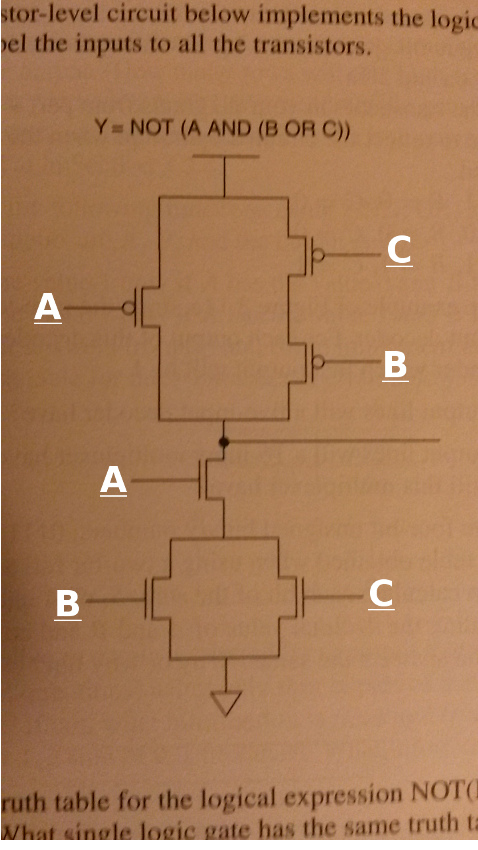
\includegraphics[width=3in]{prob8}
   \caption{Labeled Circuit for Problem \#12}
   \label{fig:prob8}
\end{figure}  

%==========================================
%========= Ch 3, #12 (1.5 pts) =============
%==========================================
\item 

%==========================================
%========= Ch 3, #21 (1.5 pts) =============
%==========================================
\item If a byte-addressable memory has 14-bit addresses, how many nibbles of storage are in this memory? \\
\textbf{Answer :} 16,384 bytes = 32,768 nibbles

%==========================================
%========= Ch 3, #23 (1.5 pts) =============
%==========================================
\item Given the logic circuit in Figure 3.38 (textbook), fill in the Z values in the truth table.
\textbf{Answer :} 
\begin{tabular}{ l | c | c | r }
  A & B & C & Z \\
  \hline 
  0 & 0 & 0 & 0 \\
  \hline
  0 & 0 & 1 & 0 \\
  \hline 
  0 & 1 & 0 & 0 \\
  \hline
  0 & 1 & 1 & 0 \\
  \hline 
  1 & 0 & 0 & 0 \\
  \hline
  1 & 0 & 1 & 0 \\
  \hline 
  1 & 1 & 0 & 0 \\
  \hline 
  1 & 1 & 1 & 0 \\
\end{tabular}

\end{enumerate}





\end{document}